\documentclass[11pt,a4paper]{article}
\usepackage[utf8]{inputenc}
\usepackage[T1]{fontenc}
\usepackage[french]{babel}
\usepackage{graphicx}
\usepackage{amsmath}
\usepackage{amssymb}
\usepackage{booktabs}
\usepackage{hyperref}
\usepackage{geometry}
\usepackage{caption}
\usepackage{subcaption}
\usepackage{float}
\usepackage{tikz}
\usetikzlibrary{positioning, arrows.meta}

\geometry{margin=2.5cm}

\title{Reconstruction 3D par Voie Tactile : Approche PointNet + SIREN}
\author{Antigravity — ISIR Stage}
\date{\today}

\begin{document}

\maketitle

\begin{abstract}
Ce rapport présente les résultats d'un modèle de reconstruction de forme 3D à partir de points de contact parcimonieux. L'architecture repose sur un encodeur PointNet pour extraire des caractéristiques globales des contacts et un décodeur SIREN pour représenter l'objet sous forme de champ de distance signé (SDF) continu. Les résultats montrent une capacité du modèle à généraliser des formes géométriques complexes à partir de seulement six points de contact.
\end{abstract}

\section{Introduction}
La reconstruction de forme à partir du toucher est un défi majeur en robotique. Contrairement à la vision, le toucher fournit des informations locales extrêmement précises (position, normale, tangente) mais très éparses. Ce projet explore l'utilisation des représentations neurales implicites (INR) pour combler cette lacune.

\section{Méthodologie}

\subsection{Architecture du Modèle}
L'architecture est composée de deux blocs principaux :
\begin{enumerate}
    \item \textbf{Encodeur PointNet} : Traite $N$ points de contact ($N=6$). Chaque point possède 9 dimensions (position $xyz$, normale $n_x n_y n_z$, tangente $t_x t_y t_z$). Un MLP partagé extrait des caractéristiques locales, agrégées par un \textit{max-pooling} pour obtenir un code latent de 256 dimensions.
    \item \textbf{Décodeur SIREN} : Un réseau à fonctions d'activation sinus qui prend en entrée une coordonnée 3D et le code latent, et prédit la valeur SDF correspondante.
\end{enumerate}

\subsection{Fonction de Perte}
La perte totale est une combinaison pondérée de trois termes :
\begin{equation}
    \mathcal{L} = \mathcal{L}_{SDF} + \lambda_{c} \mathcal{L}_{contact} + \lambda_{e} \mathcal{L}_{eikonal}
\end{equation}
Où $\mathcal{L}_{SDF}$ est la perte L1 sur les points de requête, $\mathcal{L}_{contact}$ force le SDF à zéro aux points de contact, et $\mathcal{L}_{eikonal}$ régularise le gradient pour qu'il soit unitaire.

\section{Résultats}

\subsection{Dynamique d'Entraînement}
L'entraînement a été effectué sur 50 objets de catégories variées (bouteilles, tasses, marteaux, tournevis, clés). La figure \ref{fig:training} montre l'évolution de la perte et de l'IoU.

\begin{figure}[H]
    \centering
    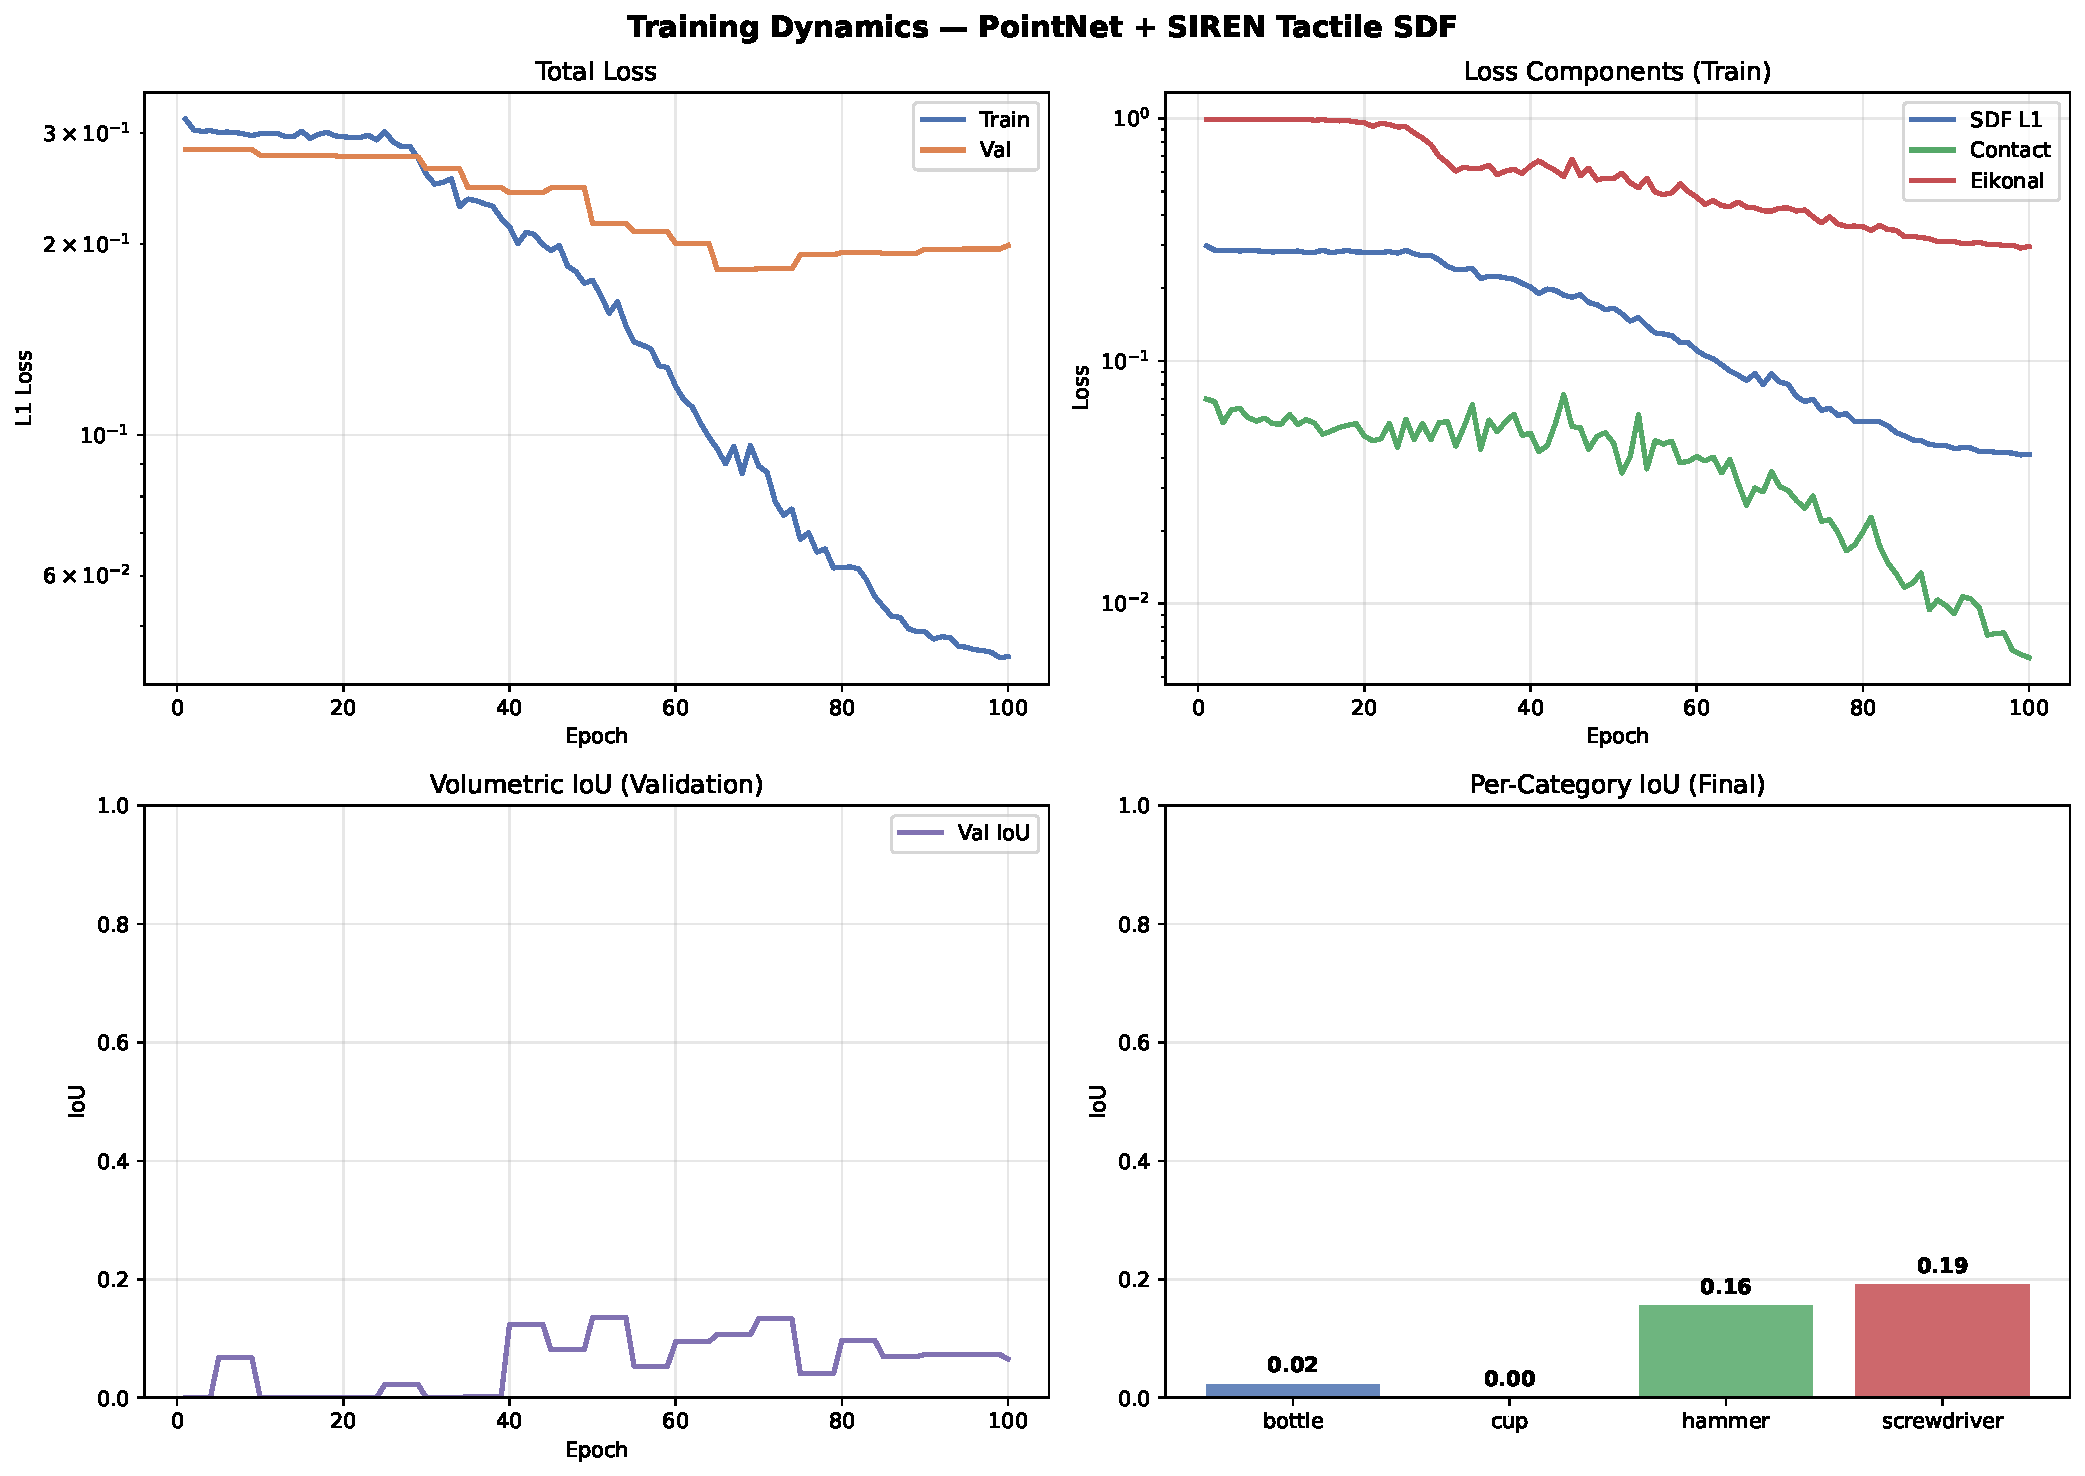
\includegraphics[width=0.8\textwidth]{figures/training_curves.pdf}
    \caption{Évolution des pertes et de l'IoU au cours de l'entraînement.}
    \label{fig:training}
\end{figure}

\subsection{Performance par Catégorie}
L'IoU varie selon la complexité géométrique des objets. Les résultats par catégorie sont présentés en figure \ref{fig:iou_cat}.

\begin{figure}[H]
    \centering
    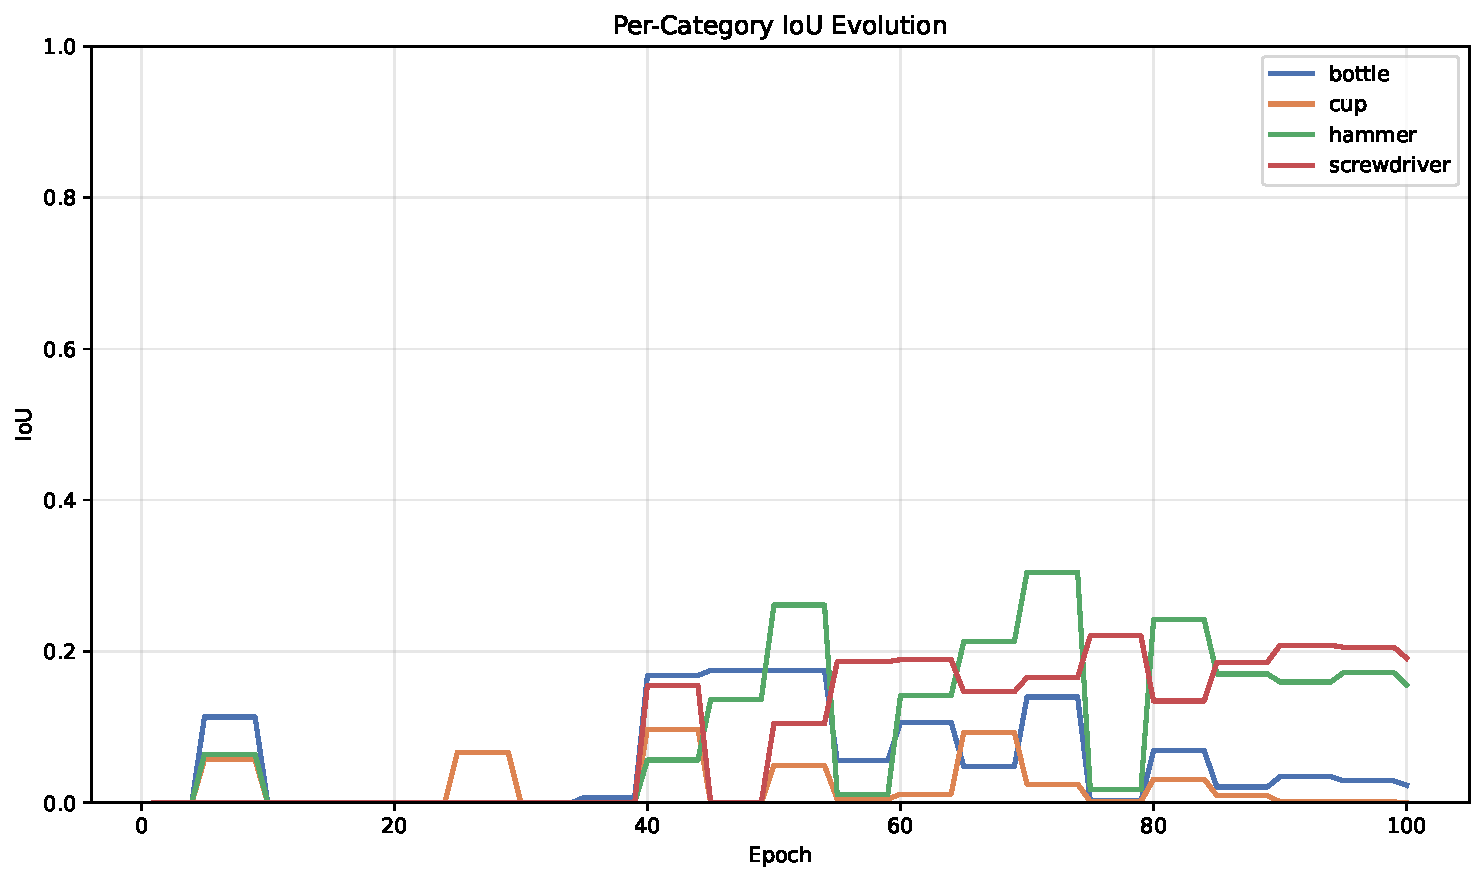
\includegraphics[width=0.8\textwidth]{figures/per_category_iou.pdf}
    \caption{Précision de reconstruction (IoU) par catégorie d'objet.}
    \label{fig:iou_cat}
\end{figure}

\section{Conclusion}
L'approche combinant PointNet et SIREN s'avère efficace pour la reconstruction tactile. Les fonctions d'activation sinus permettent de capturer des détails fins de la surface même avec une supervision éparse.

\end{document}
